\documentclass{amsart}
\usepackage{amsmath}
\usepackage{amssymb}
\usepackage{graphicx}
\usepackage{listings}
\usepackage{geometry}
\geometry{a4paper}

\title{Homework 4}
\author{Jason Medcoff}
\date{} 

\begin{document}
	\maketitle
	
	\noindent{\textbf{Question 1.}}
	a) Calculate the needs matrix. This is found by maximum demand minus current allocation.
	\begin{table}[h]
		\centering
		\caption{Problem 1 Needs Matrix}
		\label{needs}
		\begin{tabular}{l|llll}
			& $R_a$ & $R_b$ & $R_c$ & $R_d$  \\ \hline
			$P_0$ & 0     & 3     & 0     & 0     \\
			$P_1$ & 0     & 7     & 5     & 0     \\
			$P_2$ & 1     & 0     & 0     & 2     \\
			$P_3$ & 0     & 0     & 2     & 0     \\
			$P_4$ & 0     & 6     & 4     & 2    
		\end{tabular}
	\end{table}

	b)
	\begin{lstlisting}
	available = [1, 5, 2, 0]
	work = available
	done = [0, 0, 0, 0, 0]
	loop:
	    if we find i such that:
	        done[i] == 0
	        need[i] <= work
	        then
	            work = work + allocation[i]
	            done[i] = 1
	    if done[i] = 1 for all i:
	        return SAFE STATE
	\end{lstlisting}
	
%	From the algorithm, we see first that $P_3$ has needs [0, 0, 2, 0] $\leq$ work [1, 5, 2, 0], so set work = work + allocation[3] = [0, 11, 5, 2]. Next, for $P_4$, we have [0, 6, 4, 2] $\leq$ [0, 11, 5, 2], so work = [0, 11, 6, 6]
	
	From the algorithm, we see $P_0$ has needs [0, 3, 0, 0] $\leq$ [1, 5, 2, 0] so set work = [1, 5, 3, 4]. Then $P_2$ has [1, 0, 0, 2] so set work = [2, 8, 8, 8]. Now $P_1$ has needs [0, 7, 5, 0] so work = [3, 8, 8, 8]. $P_3$ has [0, 0, 2, 0] and sets work = [3, 14, 11, 10]. Finally, $P_4$ has needs [0, 6, 4, 2] so work ends at [3, 14, 12, 14]. All processes have completed, so the system is in a safe state with process sequence $P_0$, $P_2$, $P_1$, $P_3$, $P_4$.
	
%	c) The request [0, 3, 0, 0] is less than the available [1, 5, 2, 0], and is less than or equal to $P_0$'s need [0, 3, 0, 0]. So, assuming the request is accepted, available becomes [1, 2, 2, 0] and allocation becomes [0, 3, 1, 2]. Running the algorithm as in (b), we find a sequence $P_3$, $P_4$, $P_0$, $P_1$, $P_2$ supporting the safe state.
	
	$\newline$
	\noindent{\textbf{Question 2.}}
	Memory protection is important as it prevents different processes from modifying each other's memory space. For example, a C program could index an array out of bounds, or dereference a bad pointer, leading to modification of another program's memory. In a protected system, this is caught as a segmentation fault, but in an unprotected system, this could lead to undefined behaviour in the victim program.
	
	$\newline$
	\noindent{\textbf{Question 3.}}
	a) 130
	b) does not map
	c) process 1, address 250
	
	\noindent{\textbf{Question 4.}}
	1. [1, $2K-1$], [$4K$, $6K-1$]
	2. 
	\begin{enumerate}
		\item address $4500 = 4\cdot 1024 + 404$; page $4$ with offset $404$
		\item address $8000 = 7\cdot 1024 + 832$; page $7$ with offset $832$
		\item address $3000 = 2\cdot 1024 + 952$; page $2$ with offset $952$
		\item address $1100 = 1\cdot 1024 + 76$; page $1$ with offset $76$
	\end{enumerate}
	We know from 1.\ that the first virtual address will cause a page fault. According to the reference string, page 7 was least recently used and will be replaced. Its new physical address is $1\cdot 1024 + 404 = 1428$. The new table follows.
	\begin{table}[h]
		\centering
		\caption{Page table post-replacement}
		\label{page}
		\begin{tabular}{l|l|l}
			Virtual page & Physical page & Valid flag \\ \hline
			0            &               & no         \\
			1            &               & no         \\
			2            & 2             & yes        \\
			3            & 3             & yes        \\
			4            & 1             & yes        \\
			5            &               & no         \\
			6            & 0             & yes        \\
			7            &               & no        
		\end{tabular}
	\end{table}
	
	The second reference, 8000, will also fault, and considering the reference string, page 6 will be replaced. Its physical address is $0\cdot 1024 + 832 = 832$.
	\begin{table}[h]
		\centering
		\caption{Page table post-replacement 2}
		\label{page2}
		\begin{tabular}{l|l|l}
			Virtual page & Physical page & Valid flag \\ \hline
			0            &               & no         \\
			1            &               & no         \\
			2            & 2             & yes        \\
			3            & 3             & yes        \\
			4            & 1             & yes        \\
			5            &               & no         \\
			6            &               & no         \\
			7            & 0             & yes        
		\end{tabular}
	\end{table}
	
	Next, the third reference, 3000, will not fault as it does not fall in fault range. The fourth reference, 1100, will fault, and page 3 will be replaced. The physical address is $3 \dot 1024 + 76 = 3148$.
	
	$\newline$
	\noindent{\textbf{Question 5.}}
	1. $2^{24}$ bytes = 16 MB.
	2. Since offset length is 7, page size is $2^7 = 128$ bytes.
	3. $$\frac{2^{24}}{2^7} = 2^{17} = 128\ \text{KB} $$
	4. 
	99\% (normal access time) + 1\% (fault access time)
	= 99\% (99\% (TLB hit access time) + 1\% (TLB miss access time)) + 1\% (fault access time)
	= 99\% (99\% (a+b)+1\% (a+5b)) + 1\% (a+4b+c)
	\begin{equation*}
	\begin{split}
	99\% \text{(normal access time)} + 1\% \text{(fault access time)} \\
	= 99\% (99\% \text{(TLB hit access time)} + 1\% \text{(TLB miss access time)}) + 1\% \text{(fault access time)} \\
	= 99\% (99\% (a+b)+1\% (a+5b)) + 1\% (a+4b+c)
	\end{split}
	\end{equation*}
	
	$\newline$
	\noindent{\textbf{Question 6.}}
	a)
	\begin{figure}
		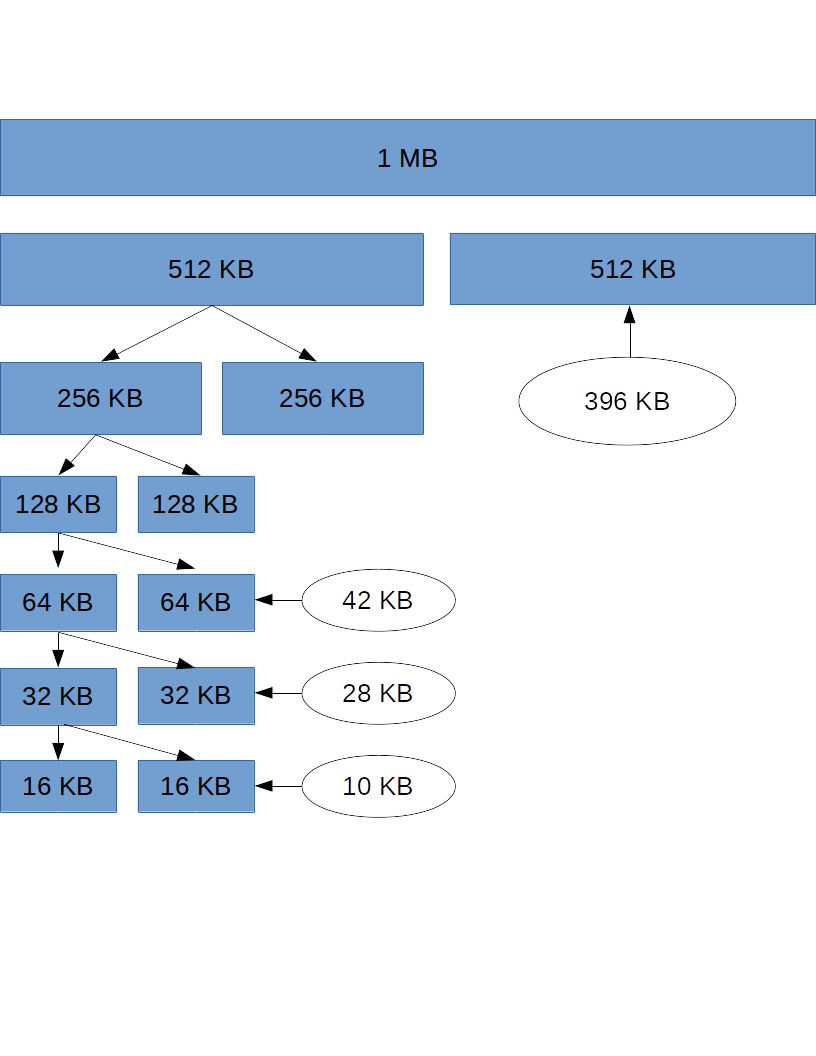
\includegraphics[scale=0.5]{diag1.png}
	\end{figure}
	
	b) Because memory is allocated in powers of two, up to half of allocated memory could end up unnecessary. Here the total is
	$$ (512-396) + (64-42) + (32-28) +(16-10) = 148 \ \text{KB}.$$
	
	c) In this algorithm, free space holes are created by the same powers of two rule. The total is
	$$ 16 + 128 + 256 = 400 \ \text{KB} $$
	so requested memory sizes greater than 256 KB cannot be granted.
	
	
	
	
	
	
	
	
	
	
	
\end{document}